\chapter{Experiment 1: Selection versus search}\label{exp1}
Disregarding what algorithm is used during path searching, training multiple machine learning models are usually rather resource intensive. In the case of training subsets of a Super Neural Network, even more so. Any small reduction in the computation time here will pay off in the long run, especially during experimentation where multiple iterations of PathNet training are going to be performed. Keeping this motivation in mind, the first experiment I performed is one where the results either confirm a shortcut in experimentation can safely be made or will give some insight into the layer interface of a model when applying different training schemes.

The questions I want to answer is simple: \textit{Is there anything to gain from performing a proper search for the first path versus just picking a random path and training those weights using a classic end-to-end training scheme?}

\section{Hypothesis}
It is self-evident that picking a random path and training that subset of weights end-to-end will be more computationally efficient than a full search through a population of possible paths. A full search in a newly initialized PathNet means we are looking for modules with the most appropriate initial weights, which is a lot of labour for a rather small amount of reward. If the change of training scheme from full search to end-to-end training is shown to not affect module reuse, subsequent experiments will be performed with end-to-end training of the first task, as this would reduce search time. What I suspect is that end-to-end training will cause the modules in the randomly chosen path to have a highly codependent interface between modules. This might then make it harder for subsequent tasks to reuse the intertwined modules, and make the encoded knowledge in those modules more task-specific than in the case of a full path-search. 

When training on two tasks, the amount of module reuse between these tasks should be lower when we end-to-end train a randomly chosen path. To test this, the following experiment is suggested. 

\section{Description}
The experiments in this section is divided in two parts. 
\begin{itemize}
    \item Search + Search (S+S): A full search for task A is performed on a newly initialized PathNet. The optimal path is saved and locked as per the PathNet design, then another full search for task B is performed.
    \item Pick + Search (P+S): A path is arbitrarily selected from the PathNet modules and trained on task A with a classic end-to-end training scheme. This path is then saved and locked normally. Then a full search is done for task B.
\end{itemize}
Performing multiple runs of this experiment should show a trend in module reuse between S+S and P+S scenarios. To ensure that the first path in P+S does not have an advantage or disadvantage in total capacity,  the path found for task A in S+S is stored and used as the arbitrarily chosen path for task A in the P+S scenario. This ensures that when training on task B in both the S+S and P+S scenario, the only difference is the weights along the path for task A, and the way these were reached. 

The MNIST set of handwritten digits is used as dataset for task A and B. This is because of the task simplicity and availability of the data set. 
It is also the same data used for the initial experiment performed on PathNet by Fernando et. al in \cite{pathnet}. Separating this implementation from \cite{pathnet} is that the data is kept as originally provided, and no additional salt and pepper noise is added to increase the task difficulty. 


I performed two experiments of this type. First, a binary classification scenario where I selected four classes from the ten available in the MNIST set and split them into two groups of two classes as task A and task B. The second experiment was a quinary classification scenario where all 10 classes were used in two groups of five each. The reason for the second experiment is discussed in the result section of experiment one. 

\section{Hyperparameters}
\label{exp1:implementation}
The implementation of PathNet has already been described in a preceding section of this thesis, so only the hyper-parameters used in the experiment will be discussed here. A list of hyper-parameters can be found in table \ref{tab:exp1.hyperparam}

\begin{table}[ht]
\centering
\begin{tabular}{lll}
                       & Binary MNIST                                                                                 & Quinary MNIST                                                                                                                                                     \\
Number of Layers       & 3                                                                                            & 3                                                                                                                                                                 \\
Number of Modules      & 10                                                                                           & 10                                                                                                                                                                \\
Module structure       & Dense only                                                                                   & Dense and Conv                                                                                                                                                    \\
Maximum active modules & 3                                                                                            & 3                                                                                                                                                                 \\
PathNet structure      & \begin{tabular}[c]{@{}l@{}}Flatten \\ Dense\\ Dense\\ Dense\\ Unique /w softmax\end{tabular} & \begin{tabular}[c]{@{}l@{}}Conv + BatchNormalization\\ Conv + BatchNormalization\\ Conv + BatchNormalization\\ Maxpool\\ Flatten\\ Unique /w softmax\end{tabular} \\
Task optimizer         & SGD                                                                                          & Adam                                                                                                                                                              \\
Learning rate          & 0.0001                                                                                       & 0.0001                                                                                                                                                            \\
Loss function          & Binary Crossentropy                                                                          & Categorical Crossentropy                                                                                                                                          \\
\# of training images   & 24754                                                                                        & 60000                                                                                                                                          \\
\# of validation images & 4157                                                                                         & 10000    

\end{tabular}
\caption{Hyperparameters used in the first-path experiments. A Dense module here consists of 20 fully connected nodes with ReLU activation, while a convolutional module is 1 channel of a 3-by-3 kernel with 1-by-1 stride and ReLU activation.}
\label{tab:exp1.hyperparam}
\end{table}

\section{Binary MNIST classification}
\label{exp1:results.binary}

\subsection{Experimental setup}
A similar PathNet structure to the MNIST experiment in the original PathNet paper is used here. 
Three layers with a maximum of three active modules from a total of 10, each with 10 fully connected nodes followed by ReLU-activation. Since each data point in MNIST is a 28 by 28 grey scale picture, the matrix of input-values is first flattened to a 784-element vector before it is used in training. The digits 3 and 4 were selected as task A, and digits 1 and 2 as task B. 
During the search, a population of 64 paths were used, and the search halted when a training accuracy of 98\% was reached, or after 500 generations. During tests, searches that exceeded 500 generations usually persisted for more than 1000 generations because the training was stuck in a local-minima. The population had always converged to one path at that point, and excessive training on a converged path would after a while approximate end-to-end training. Because of this and limitations to available experimentation time, the limit of 500 generations is enforced. The task-specific classification layer that is used alongside the PathNet weights is obviously restricted by the training scenario and its use, so it consists of two fully connected nodes followed by Softmax-activation for the purpose of classification.
A total of 600 experimental runs were performed.


\subsection{Results}
\label{exp1:BIN.results}
\begin{figure}[t]
    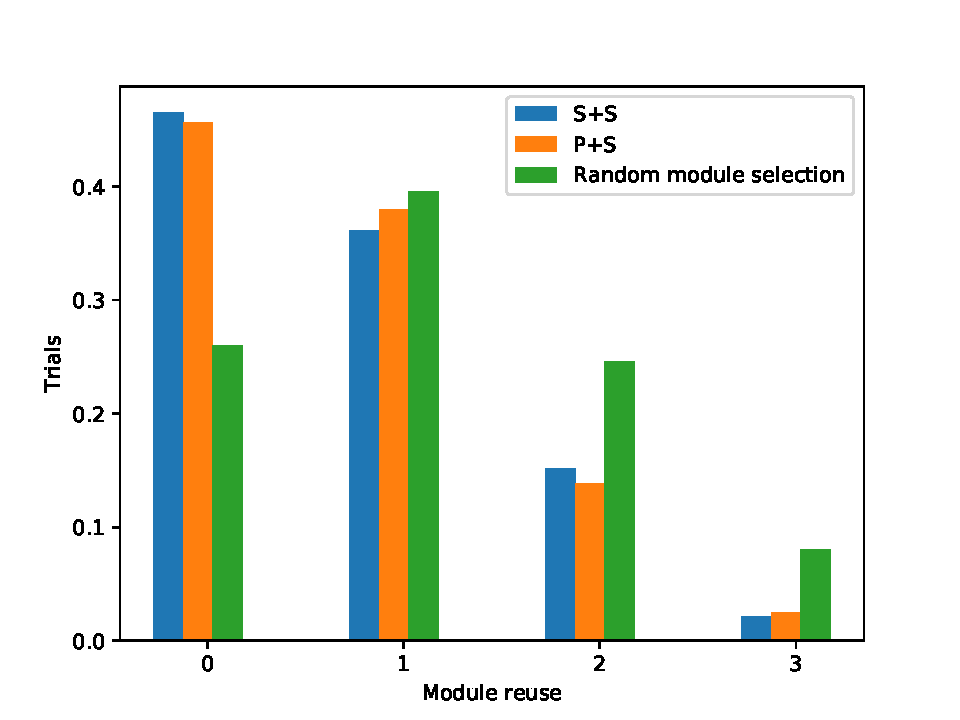
\includegraphics[width=\textwidth]{Chapters/4.Experiments/exp1/figures/BIN_module_reuse_bargraph.pdf}
    \caption[Module reuse for binary MNIST classification]{Distribution of module reuse in S+S and P+S searches alongside expected module reuse for random selection of modules in first and second task[green]. This plot is a result of 600 experimental runs.}
    \label{fig:binMNIST.hist}
\end{figure}

The amount of module reuse between the two tasks is visualized in three plots in terms of frequency, training and layer-distribution.

Figure \ref{fig:binMNIST.hist} shows a bar graph of how the amount of trial are distributed on the different amounts of reuse achieved. Compared to the S+S and P+S training schemes, the expected distribution of trials for random module selection is plotted in green. No difference between S+S and P+S for any of the reuse amount is observed here, however, the amount of trials where zero reuse were found is significantly higher than expected from random module selection. Performing a Mann-Whitney rank-sum test for the two groups of module reuse show not significant difference between selecting the first path arbitrarily or searching for it with tournament search. 

\begin{figure}[t]
    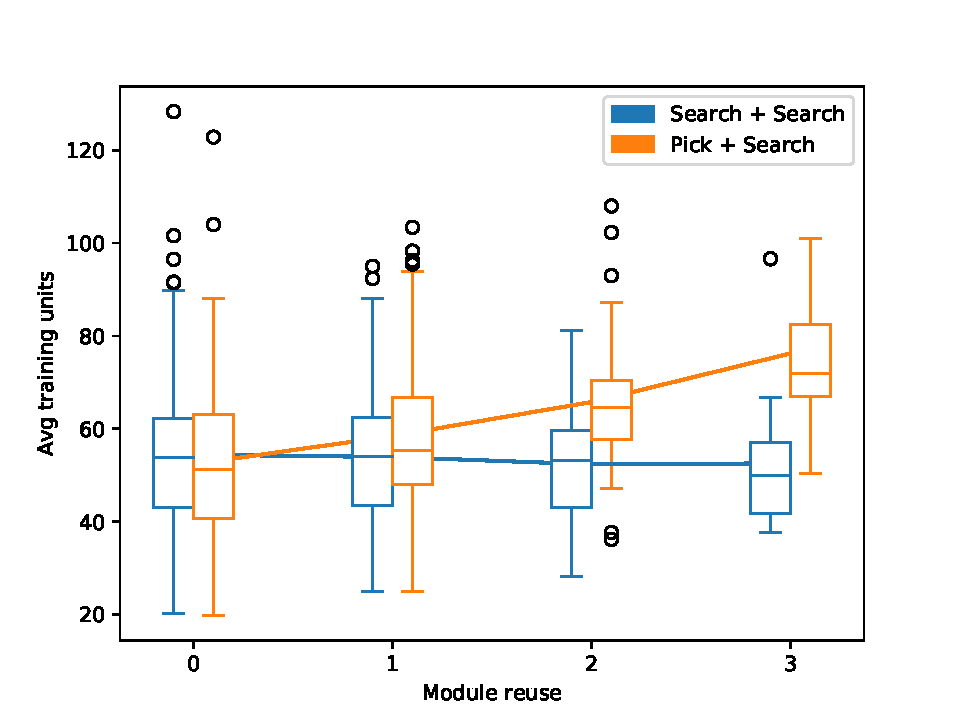
\includegraphics[width=\textwidth]{Chapters/4.Experiments/exp1/figures/BIN_training_boxplot.pdf}
    \caption[Training boxplot for binary MNIST classification]{Box-plot depicting average amount of training each module within a path gets for each group of module reuse for both P+S and S+S. Note that as the module reuse increase, the number of observations in each group decrease. Figure \ref{fig:binMNIST.hist} visualize the difference in group size.}
    \label{fig:binMNIST.box}
\end{figure}

The average amount of training units\footnote{Each module in a path undergoes one unit of training when that path is evaluated once during a search. In this case that means 50 mini-batches of size 16.} each module in the optimal path found for task B is plotted against reuse in figure \ref{fig:binMNIST.box}. It is clear here that paths with a higher amount of reuse also have a higher amount of average training when the first path have arbitrarily been selected. The S+S scheme on the other hand, does not seem to have any significant change in average training across the different reuse groups. 

A series of Mann-Whitney tests for each group of reuse found in figure \ref{fig:binMNIST.box} shows there is no difference in average training units for zero reuse between S+S and P+S, while the difference for 1 module reuse and higher is statistically significant under a Bonferroni corrected significance level of \(\frac{0.05}{4}=0.0125\).

\begin{figure}[t]
    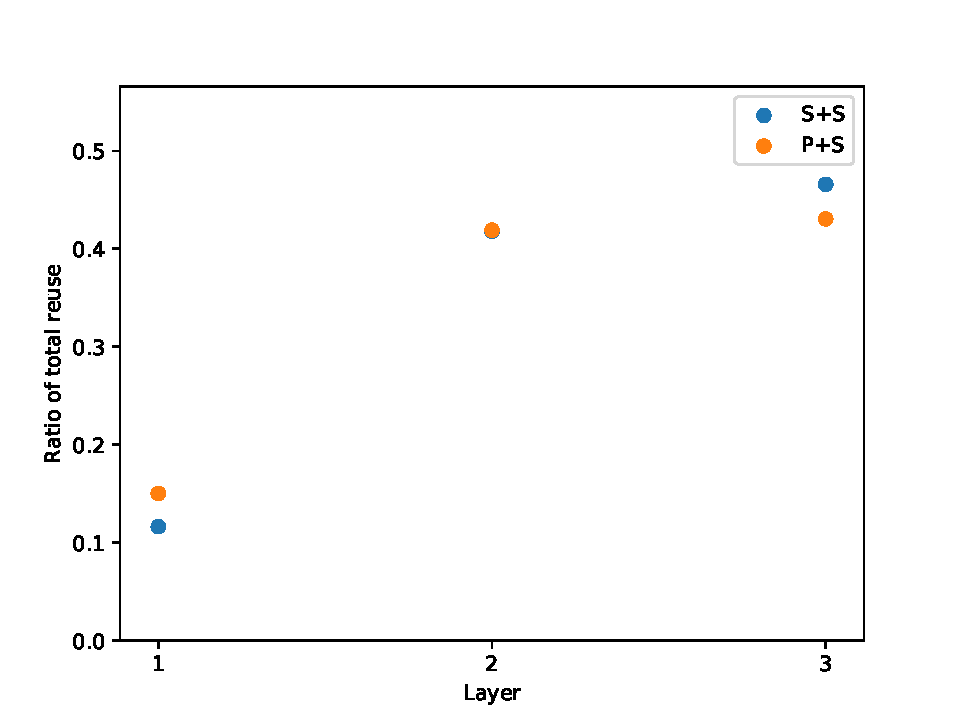
\includegraphics[width=\textwidth]{Chapters/4.Experiments/exp1/figures/BIN_reuse_by_layer.pdf}
    \caption[Reuse by layer for binary MNIST classification]{This plot shows how the total amount of reuse in all experiments are distributed on the three layers in the PathNet structure }
    \label{fig:binMNIST.layer_reuse}
\end{figure}
 
The total amount of reuse found across all experimental trials are split into which layer they occur in for figure \ref{fig:binMNIST.layer_reuse}. While the difference between S+S and P+S is small, the difference between layers is quite prominent. The first layer contain significantly less of the total reuse amount at about 10-15\%. The rest of the reuse are about evenly split on the last two layers, making the distribution quite uneven. 


\subsection{Discussion}
\label{exp1:BIN.discussion}
The hypothesis stated in the beginning of this chapter would manifest itself in figure \ref{fig:binMNIST.hist} as a higher total amount of reuse for S+S than P+S. The observations does not fit under the hypothesis that end-to-end training causes confounded interfaces between layers as the two distributions seem to be equal. However, as the amount of trials with no reuse is significantly higher than expected, it might seem like the task used is to simple. This would cause the paths to train very little and the available capacity in the paths to be too high. When the distance in parameter space between initialize parameters and "good enough" parameters are too small, the gain from reusing modules can not be justified. In other words, learning the task \textit{de novo} is simpler than learning the interface-quirks of a preceding previously used module. In that case there would be no difference between selecting the first path arbitrarily and searching for it with a tournament search. 

As these searches are limited by a threshold accuracy, P+S might reach the same accuracy and reuse results as S+S but need more training units to get there. This is what is observed in figure figure \ref{fig:binMNIST.box} where the separation between S+S and P+S is striking. Had these experiments been limited by number of generations the tournament search is performed for, there might have been a difference in reuse in figure \ref{fig:binMNIST.hist}.

As discussed in section \ref{background:TL} the first layer in a trained NN tend to be the most generalized as the low level feature extraction performed by these layers are the same for most image classification. The opposite seems to be the case in these experiments, as figure \ref{fig:binMNIST.layer_reuse} would indicate. This is most likely a property of using multi-layer perceptrons as modules and would disappear if the modules in question consisted of convolutional operations. Fully connected NNs are poor at generalizing to image data because of images complex class manifolds and as a result of the raw image processing most CNN's end up performing in their first layers, convolutional layers that approximate Gabor-filters ends up being highly transferable\cite{yosinski2014transferable}.

What we see instead is that most module reuse happens in later layers in the PathNet. It is hard to tell exactly why this is, but a possible explanation is that a path contains more capacity than it needs and the later layers are capable of doing all the heavy lifting. In that case, the first layer does not contain use full weights, and therefore there is no incentive to reuse those modules. 

Since this implementation is one of fully connected nodes, each neuron has to generalize to its corresponding image pixels, and would therefore be highly task specific. This is the motivation behind performing the quinary MNIST classification experiment in addition to this one. More classes constitute a "harder" classification task, and the change from NNs to CNN's as modules should remove some of the effects we have seen in the plots in this section. Effects we expect to see in Quinary MNIST classification is

\begin{enumerate}
    \item A separation between P+S and S+S in the frequency of models with a higher module reuse.
    \item S+S should have a frequency distribution closer to the distribution by randomly choosing modules.
    \item A significantly smaller divergence between P+S and S+S in average training for each module reuse group. 
    \item A more even distribution of module reuse on each layer in a path.
\end{enumerate}

Point 4 because the modules are changed from NNs to CNNs, and 1 through 3 because we increase the task difficulty and therefore also the necessary training time. 

\section{Quinary MNIST classification}
\subsection{Experimental setup}
A different PathNet structure was implemented here. The first two layers consisted of 10 convolutional modules each, where a convolutional module contained two convolutional layers, the first with a 3 by 3 kernel and ReLU activation, and the second with a 5 by 5 kernel and ReLU activation. Following these convolutions, a Batch-Normalization layer is added to reduce the spread in gradients. The third and last PathNet-layer were 10 modules of 20 fully connected nodes and another ReLU activation. To connect the second and third layer, a two-dimensional Maxpooling reduced the dimensionality of the second layers output before the 2D matrix was flattened to a vector.   

The path searches were again done with a population of 64 paths and a limitation of 500 generations, but the threshold training accuracy used here were 97.5\% to limit run time. 
Since the classification task here were quinary and all 10 classes from the MNIST set were used, for simplicity's sake, task A consisted of digits 0 through 4, and digits 5 through 9 made up task B. 

This experiment was considerably more computationally expensive to run, so it was programmed to keep running until no more time could be dedicated to this experiment. In the end, this ended up being 535 experiments. 

\subsection{Results}
\label{exp1:results.quinary}
Each of figures in section \ref{exp1:BIN.results} have their Quinary MNIST counterpart here, but included in these plots are a version of the S+S scheme called S+S flipped\footnote{In S+S, task A consisted of classifying the classes \{0, 1, 2, 3, 4\} while task B were classes \{5, 6, 7, 8, 9\}}, where the task order have been reversed.

\begin{figure}[t]
    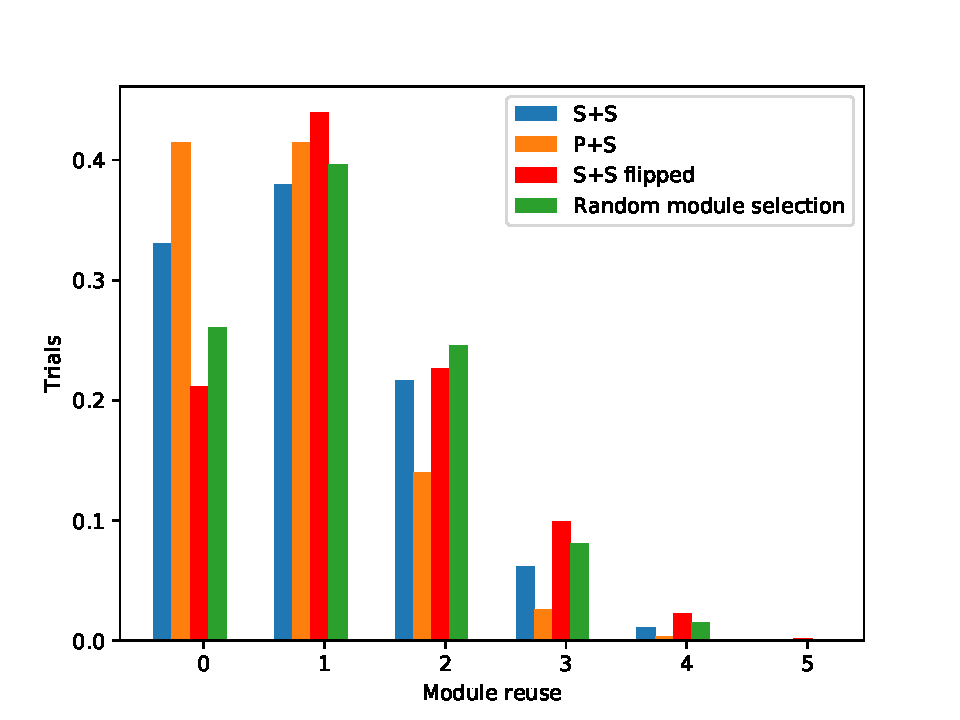
\includegraphics[width=\textwidth]{Chapters/4.Experiments/exp1/figures/QUIN_module_reuse.pdf}
    \caption[Module reuse for quinary MNIST classification]{Frequency histogram equivalent to \ref{fig:binMNIST.hist} for the Quinary MNIST classification experiment. The red bar shows reuse in a training scenario similar to S+S, but where the order of tasks is reversed.}
    \label{fig:quinMNIST.hist}
\end{figure}

\begin{figure}[t]
    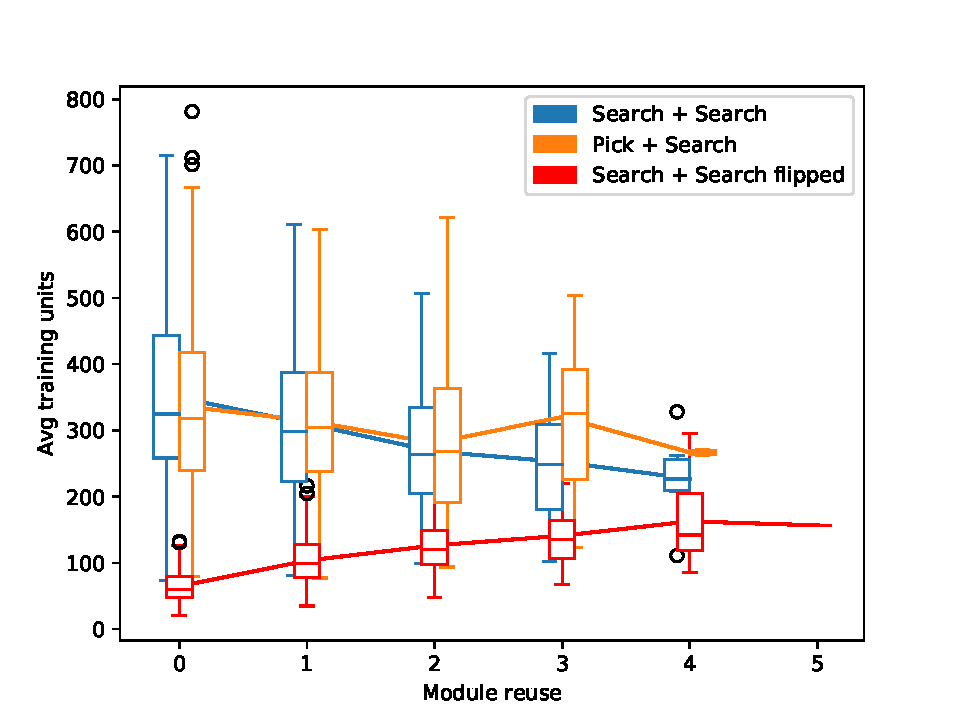
\includegraphics[width=\textwidth]{Chapters/4.Experiments/exp1/figures/QUIN_training_boxplot.pdf}
    \caption[Training boxplot for quinary MNIST classification]{Average training box-plot equivalent to \ref{fig:binMNIST.box} except for the addition of a training scenario similar to S+S but where the task order is reversed. Note that as the module reuse increase, the number of observations in each group decrease. Figure \ref{fig:quiMNIST.hist} visualize the difference in group size.}
    \label{fig:quinMNIST.box}
\end{figure}

\begin{figure}[t]
    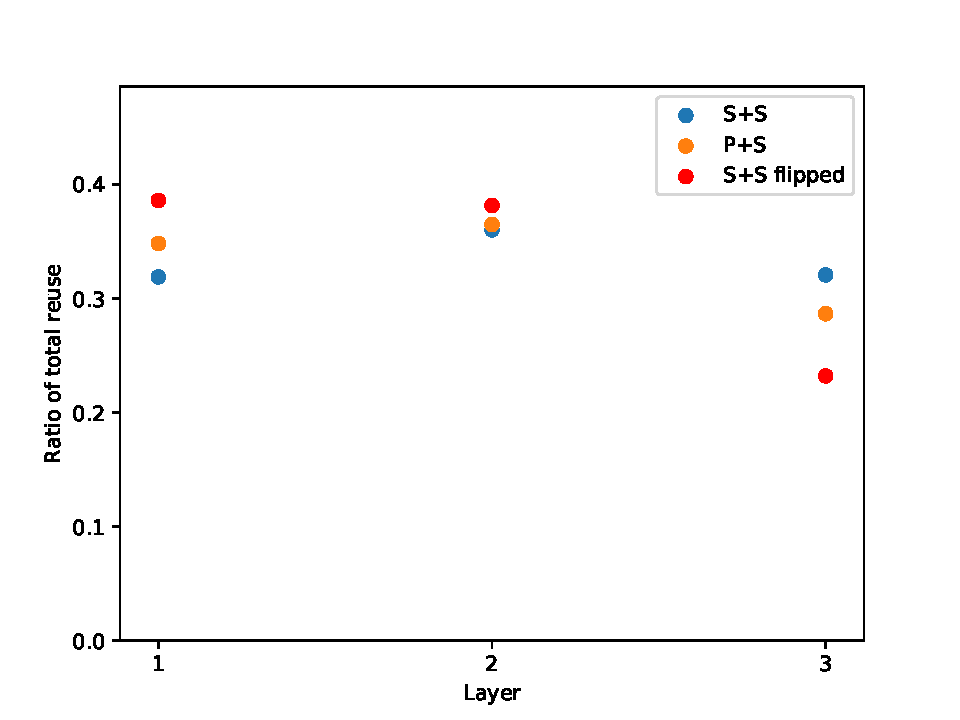
\includegraphics[width=\textwidth]{Chapters/4.Experiments/exp1/figures/QUIN_reuse_by_layer.pdf}
    \caption[Reuse by layer for quinary MNIST classification]{Frequency of module reuse for each layer in the paths. Equivalent to \ref{fig:binMNIST.layer_reuse} except for the addition of a training scenario similar to S+S but where the task order is reversed}
    \label{fig:quinMNIST.layer_reuse}
\end{figure}

It is quickly eminent from figures \ref{fig:quinMNIST.hist} and \ref{fig:quinMNIST.box} that the increase in task difficulty between binary MNIST and quinary MNIST have uncovered effects predicted in the original hypothesis. In the bar graph \ref{fig:quinMNIST.hist}, a clear difference between P+S and S+S is visible and confirmed with Mann-Whitney testing. This difference is even more prominent for S+S flipped, but as these trials have a different task order and the information contained in task B might be harder or easier to generalize, the comparison between S+S flipped and P+S is not entirely fair. 

The difference between S+S and P+S in figure \ref{fig:binMNIST.box} are not present in figure \ref{fig:quinMNIST.box}. Instead a downward trend in average training for paths with a higher reuse have emerged. To test why this is, S+S flipped have been introduced and paths learning task B first have a trend where average training increase for a higher amount of reuse. Over-all, the training for paths trained in S+S flipped is also significantly lower for all levels of reuse. Note also that the amount of training for S+S and P+S have increase from the binary MNIST classification which is to be expected due to the increase in task difficulty. 

Performing Mann-Whitney tests of S+S and P+S for the different reuse groups provides no rejected null-hypotheses proving there is no significant difference in average training between selecting and searching for the first path. Testing the difference between S+S and S+S flipped shows a significant difference for all groups but that of 4 module reuse. 

Figure \ref{fig:quinMNIST.layer_reuse} shows the uneven distribution across layers in figure \ref{fig:binMNIST.layer_reuse} is gone. For S+S flipped, the most amount of reuse is found in the two first layers.

\subsection{Discussion}
While the results in figure \ref{fig:quinMNIST.hist} does not hold conclusive evidence of the interface confounding predicted, the effect shown here is strong enough to discourage the end-to-end training of a chosen first path. We saw in the results for binary MNIST classification, that the amount of paths with no reuse were significantly higher than expected, but this effect seem to have disappeared for S+S where it seem about the same, while S+S flipped have surpassed random module selection in reuse. Point 1 and 2 from the list of predictions there seem to have been confirmed. 

Point 3 in the same list seem to have found conformation in figure \ref{fig:quinMNIST.box}, but this plot also introduce the decrease in average training for higher levels of reuse. This effect can be explained if we suspect the task used for the first path in each experiment to be easier than the second. Say task A in a two task system is much simpler than task B. After optimal path for task A have been found and locked, the PathNet will consist of most modules with no training, while those along path A will have a small amount. If task B is harder and more training is done during the search for path B, more reuse of modules means a higher amount of modules in path B have been trained during task A and therefore have received less training in total. The average amount of training for task B will then be lower for higher levels of reuse. 
The opposite will be true if task A is harder than task B. More reuse of modules with more training means the average training for task B will go up for higher levels of reuse. 

S+S flipped is introduced to test this, and the red boxes confirm this suspicion. While the later boxes for these results also contain a smaller amount of observation, there is undeniably a opposite trend for this task order. The over-all lower training amount might be explained the same way. If task B (classes 5, 6, 7, 8 and 9) are harder to learn, it stands to reason that it might contain more information that can be generalized to other tasks, and to generalize to that information demands a higher training effort. When S+S flipped then trains on the simple task A last, most modules in the optimal paths found did not need to undergo the same amount of training effort, meaning the average path for S+S flipped have a lower average training amount. However, the cause for this is not conclusive. 

The change from fully connected modules to convolutional modules seem to have provided results closer to what we would expect when considering results in \cite{yosinski2014transferable}. Figure \ref{fig:quinMNIST.layer_reuse} shows S+S flipped having significantly higher reuse for the first two layers which might mean these have approximated some form of Gabor-filter. Point 4 in the quinary-MNIST predictios also see confirmation here, as S+S and P+S seem to have the same reuse distribution. 

\section{Conclusion}
In conclusion, results in quinary MNIST classification as well as the comparison with the binary MNIST experiment show promising, if not conclusive, evidence of end-to-end training causing confounded interfaces between modules and a reduction in transferability between tasks in a multitask scenario. Note should also be taken of how task difficulty effect reuse, and ordering of task from low difficulty and upwards will manifest as a lower average training for paths with a high level of reuse. Results in figure \ref{fig:quinMNIST.hist} tells us there might be something undiscovered and unexpected hidden in the ordering of tasks, and further experiments are called for to uncover this. 

The motivation for these experiments was the possibility of reducing experimentation time by not searching for the first path in the PathNet structure, but the reduction in transferability is dissuading enough to not justify forgoing a full search for all paths. 

